\documentclass{beamer}
\usetheme{Madrid}
\usecolortheme{beaver}

\logo{
\includegraphics[width=1cm]{1200px-King's_College_London_logo.svg.png}}

\title{Progress Slides II (27th Feb 24)}
\author{Oscar Moxon}
\institute{King's College London}

\begin{document}

\begin{frame}
\titlepage
\end{frame}

\logo{}
\begin{frame}
\frametitle{Introduction to Multi-Agent Debate System}
\vspace{-0.3cm} % Adjust the value as needed
\begin{center}
Developing a multi-agent debate system with narrative judgement to develop c-factor in LLM agent collectives. 
This agent cluster is part of an operative kernel that could be used to bring embodied agents as a force within the workforce.
\end{center}

\begin{columns}[T] % Align content at the top

    % Left column for text
    \begin{column}{0.5\textwidth}
            \begin{itemize}

            \item[1.] Goal Identification: Identifying the objective or desired outcome.
            \item[2.a] Research \& Information Gathering: Collecting relevant data and information.
            \item[2.b] Research Execution.
            \item[3.a] Debate Staging.
            \item[3.b] Multi-Agent Debate Protocol.
            \item[4+] Out of scope.
        
            \end{itemize}

    \end{column}
    
    % Right column for the diagram
    \begin{column}{0.5\textwidth}
    \vspace{-0.6cm} % Adjust the value as needed

        \begin{figure}
            \centering
            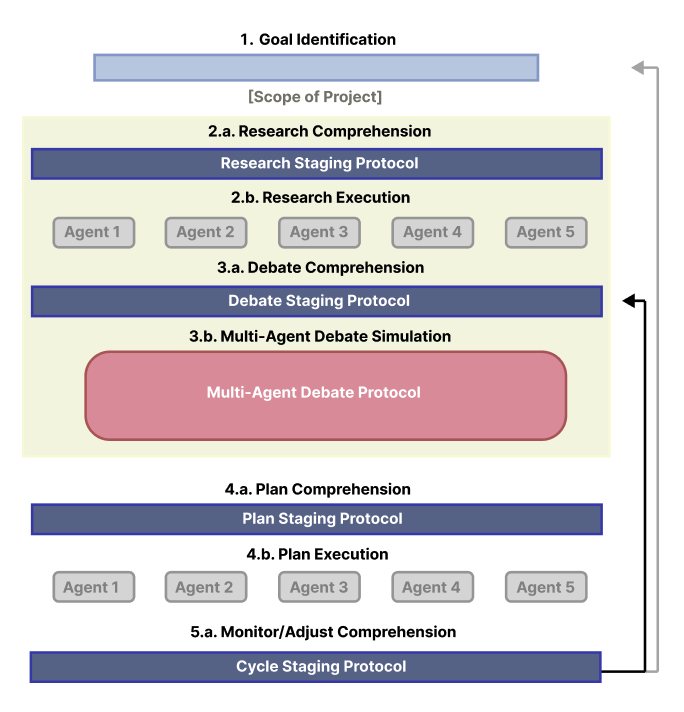
\includegraphics[width=\textwidth]{MAD-stages.png}
            \caption{Problem Solving Network}
        \end{figure}
    \end{column}

\end{columns}
\end{frame}


\logo{
\includegraphics[width=1cm]{1200px-King's_College_London_logo.svg.png}}

\begin{frame}
\frametitle{2. Research Staging Protocol}
\vspace{-0.5cm} % Adjust the value as needed to decrease or increase the space
\begin{center}
    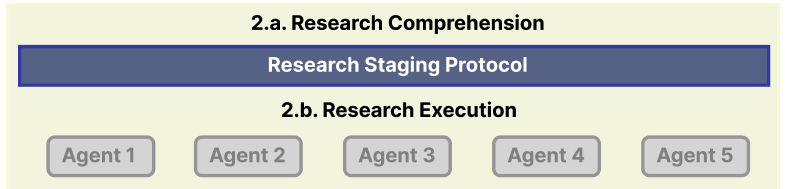
\includegraphics[width=0.5\textwidth]{MAD-stage-2.png}
\end{center}

\vspace{-0.3cm} % Adjust the value as needed
\begin{columns}[T] % The [T] option aligns the columns' content at the top
    \begin{column}{0.5\textwidth}
        \small % This command will make the text smaller
        \textbf{2.a. Task Assignment:}
        \begin{itemize}
            \item Agents are assigned specific tasks based on their designed capabilities, such as web navigation, sitemap retrieval, API interfacing, and database querying.
            \item Web navigation agents use tools like Selenium or Puppeteer for automated browsing.
            \item Sitemap and API agents may utilise HTTP requests to fetch data from predefined endpoints.
        \end{itemize}
     \end{column}
        
     \begin{column}{0.5\textwidth}
     \small
        \textbf{2.b. Parallel Execution:}
        \begin{itemize}
            \item Each agent operates in a parallel channel to ensure the gathering phase is concurrent, reducing the overall time for data collection.
            \item Agents should have asynchronous capabilities to handle I/O operations efficiently.
        \end{itemize}

    \end{column}
\end{columns}
\end{frame}



\begin{frame}
\frametitle{3.a. Debate Staging Protocol}
\vspace{-0.5cm} % Adjust the value as needed to decrease or increase the space
\begin{center}
    
\includegraphics[width=0.7\textwidth]{MAD-stage-3a.png}
\end{center}
\vspace{-0.3cm} % Adjust the value as needed

\textbf{3.a. Data Handling and QA:} 
\small
    \textbf{Agents preprocess the gathered data to normalise and structure it for downstream use.}
    \begin{itemize}
        \item Extracted data should be stored in a centralised data warehouse with a consistent schema for easy access and analysis.
        \item Implement checksums, data validation, and verification processes to ensure integrity and accuracy.
        \item Integrate cross-referencing functions where agents can compare and validate information against multiple sources.
    \end{itemize}

\textbf{Scope for Debate Coordination} 
\small
    \begin{itemize} 
        \item This stage would establish the framework for the debate, defining the roles of the judge or guide, which would be an overarching model or system designed to moderate the debate.
    \end{itemize}
\end{frame}



\begin{frame}
\frametitle{3.b. Multi-Agent Debate}

% Columns environment
\begin{columns}[T] % The [T] option aligns the content at the top of the columns

    % Left column
    \begin{column}{.48\textwidth}
        \textbf{Exploration into Inquiry dialogues in multi-agent systems}
        % Include the left part of the image here
        % Use a cropped version of the image that only contains the left half
    \end{column}

    % Right column
    \begin{column}{.48\textwidth}
        % If the right side of the image contains different content,
        % you can include additional text or another image here.
        % For now, I'm assuming it's the right half of the same image.
        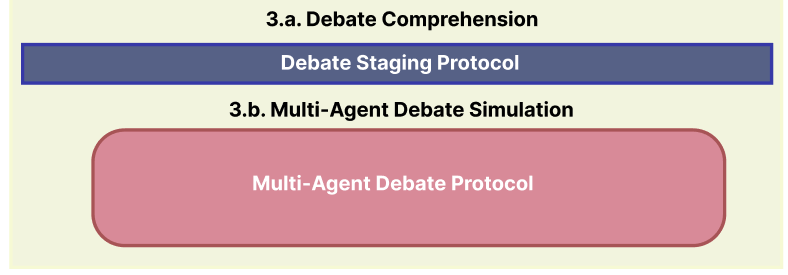
\includegraphics[width=\textwidth]{MAD-stage-3.png}
    \end{column}
\end{columns}

% Centered section
\vspace{0.5cm} % Adjust the value as needed
    \textbf{Collective Intelligence "c-Factors":} 
        \begin{itemize}
        \item \textbf{Model Size:} Larger models may provide more nuanced arguments due to their capacity for complex understanding and generating emergent behaviours.
        \item \textbf{Model Persona:} Tailoring personas for different models to represent varied perspectives and expertise.
        \item \textbf{Model Contributions:} Establishing protocols for how models interject, support, or oppose arguments, and how they build upon each other's contributions.
    \end{itemize}

\end{frame}

\logo{} % Temporarily disable the logo for this frame

\begin{frame}
\frametitle{Challenges and Measure of Success}
\small % This command will reduce the font size for the content within the scope

\textbf{Challenges:}
\begin{itemize}
    \item \textbf{Mitigating Groupthink:} Ensuring diversity in model reasoning to avoid uniformity of thought; possibly by using a diverse set of models or incorporating adversarial models.
    \item \textbf{Iterative Improvement:} Keeping the debate dynamic with new information or perspectives; perhaps through real-time updates or iterative rounds of argumentation.
    \item \textbf{Circulation of Information:} Efficiently managing how information is shared among models to inform arguments.
\end{itemize}

\textbf{Measure of Success:}
\begin{itemize}
    \item Success measured by the ability of the debate to produce a coherent narrative report that functions like a literature review, documenting debate evolution, supporting final consensus.
    \item Group c-factors then compared by these reports, with information input as a constant. Allows conclusions to be drawn about quality multi-agent debates.
\end{itemize}

\end{frame}



\begin{frame}[allowframebreaks]
\frametitle{References}
\begin{thebibliography}{10}
\small
\vspace{-0.8cm} % Adjust the value as needed

    \bibitem{Shoham2008}
    Shoham, Y. \& Leyton-Brown, K.
    \newblock \textit{Multiagent Systems: Algorithmic, Game-Theoretic, and Logical Foundations}.
    \newblock Cambridge University Press, 2008.
    
    \bibitem{Russell2010}
    Russell, S. \& Norvig, P.
    \newblock \textit{Artificial Intelligence: A Modern Approach}, 3rd ed.
    \newblock Prentice Hall, 2010.
    
    \bibitem{Mehrabi2019}
    Mehrabi, N., et al.
    \newblock ‘Bias and Fairness in the Age of Artificial Intelligence’.
    \newblock \textit{Electronics}, 8(8):835, 2019.
    
    \bibitem{Sutton2018}
    Sutton, R. S. \& Barto, A. G.
    \newblock \textit{Reinforcement Learning: An Introduction}, 2nd ed.
    \newblock The MIT Press, 2018.
    
    \bibitem{Rahwan2009}
    Rahwan, I. \& Simari, G. R.
    \newblock \textit{Argumentation in Artificial Intelligence}.
    
    \bibitem{Bordini2007}
    Bordini, R. H., Hübner, J. F. \& Wooldridge, M.
    \newblock \textit{Programming Multi-Agent Systems in Agentspeak using Jason}.
    \newblock Wiley, 2007.
\end{thebibliography}
\end{frame}

\begin{frame}[allowframebreaks]
\frametitle{Further Reading}
\begin{itemize}
    \item Bansal, S. and Weld, D.S. (2021). Chain of Thought Reasoning.
    \item Hendrycks, D. et al. (2022). Language Models as Few-Shot Common-sense Learners.
    \item Lu, S. et al. (2022). Enhancing Reasoning in Language Models.
    \item OpenReview (n.d.). Improving Reasoning in LLMs through Prompting Techniques.
    \item Prystawski, B. and Goodman, N.D. (2023). The Role of Experience in Reasoning.
    \item WebGPT, K. et al. (2023). Language Models Learning to Utilize Tools.
    \item Yao, F. (2022). Tracing GPT's Emergent Abilities.
\end{itemize}
\end{frame}

\end{document}